% Gabarit pandoc des corrigés publiés (brut et guidé). Contenu sans marque ni nom de site.
% Compilation : lualatex (latexmk -lualatex).
% Le Markdown reste la source unique : ne pas éditer ce fichier .tex à la main.
\documentclass[11pt,a4paper]{article}

% --- Moteur, polices (Latin Modern) et langue ---------------------------------
\usepackage{iftex}
\ifLuaTeX\else\errmessage{Ce document se compile avec lualatex}\fi
\usepackage{amsmath,amssymb,mathtools}
\usepackage{fontspec}
% mathrm=sym : \mathrm prend ses glyphes dans la police mathématique (ℓ, μ, Ω), comme KaTeX.
\usepackage[math-style=TeX,bold-style=TeX,mathrm=sym]{unicode-math}
% Repli pour les glyphes absents de Latin Modern (indices et exposants Unicode,
% flèches, filets des schémas en texte, symboles) : DejaVu, puis Latin Modern Math
% (ℓ, lettres mathématiques Unicode des légendes).
\directlua{
  luaotfload.add_fallback("repliTexte", {"DejaVuSerif:mode=harf;", "DejaVuSans:mode=harf;", "file:latinmodern-math.otf:mode=harf;"})
  luaotfload.add_fallback("repliMono", {"DejaVuSansMono:mode=harf;", "DejaVuSans:mode=harf;", "file:latinmodern-math.otf:mode=harf;"})
}
\setmainfont{Latin Modern Roman}[RawFeature={fallback=repliTexte}]
\setsansfont{Latin Modern Sans}[RawFeature={fallback=repliTexte}]
\setmonofont{Latin Modern Mono}[RawFeature={fallback=repliMono}]
\setmathfont{Latin Modern Math}
\usepackage[french]{babel}
\frenchsetup{SmallCapsFigTabCaptions=false}

% --- Mise en page --------------------------------------------------------------
\usepackage[a4paper,margin=2.2cm,headheight=14pt,footskip=1.2cm]{geometry}
\usepackage{microtype}
\setlength{\emergencystretch}{4em}
\tolerance=1500
\setlength{\parindent}{0pt}
\setlength{\parskip}{0.55\baselineskip plus 2pt minus 1pt}
\usepackage{xcolor}
% Gris nommés : babel-french rend « ! » actif dans le document.
\definecolor{gris2}{gray}{0.98}
\definecolor{gris3}{gray}{0.97}
\definecolor{gris5}{gray}{0.95}
\definecolor{gris35}{gray}{0.65}
\definecolor{gris40}{gray}{0.60}
\definecolor{gris45}{gray}{0.55}
\definecolor{gris50}{gray}{0.50}
\definecolor{gris55}{gray}{0.45}
\definecolor{gris60}{gray}{0.40}
\definecolor{gris65}{gray}{0.35}
\definecolor{gris70}{gray}{0.30}
\definecolor{gris80}{gray}{0.20}
\definecolor{gris85}{gray}{0.15}
\usepackage{graphicx}
\usepackage{float}
\usepackage{caption}
\captionsetup{font=small,labelformat=empty,justification=centering}
\usepackage{booktabs,longtable,array,multirow,calc}
\usepackage{siunitx}
\sisetup{locale=FR}
\usepackage[version=4]{mhchem}
\usepackage{listings}
\usepackage{fancyhdr}
\usepackage{lastpage}
\usepackage[most]{tcolorbox}
\usepackage{enumitem}
\setlist{nosep,leftmargin=*,topsep=2pt}
\usepackage[hidelinks,unicode]{hyperref}
\usepackage{bookmark}
\hypersetup{pdftitle={e3a-Polytech MPI — Mathématiques 2026},pdfauthor={Rédigé par IA},pdfcreator={LaTeX},pdfsubject={Corrigé guidé}}
\usepackage{xurl}

% --- Pandoc : listes, tableaux, figures ----------------------------------------
\providecommand{\passthrough}[1]{#1}
\providecommand{\tightlist}{\setlength{\itemsep}{0pt}\setlength{\parskip}{0pt}}

\makeatletter
\def\maxwidth{\ifdim\Gin@nat@width>\linewidth\linewidth\else\Gin@nat@width\fi}
\def\maxheight{\ifdim\Gin@nat@height>0.55\textheight 0.55\textheight\else\Gin@nat@height\fi}
\makeatother
\setkeys{Gin}{width=\maxwidth,height=\maxheight,keepaspectratio}
\setcounter{secnumdepth}{-\maxdimen}
\providecommand{\pandocbounded}[1]{#1}

% --- Code (listings) -----------------------------------------------------------
\lstset{
  basicstyle=\ttfamily\small,
  columns=fullflexible,
  keepspaces=true,
  breaklines=true,
  breakatwhitespace=false,
  postbreak=\mbox{\textcolor{gris50}{$\hookrightarrow$}\space},
  frame=single,
  rulecolor=\color{gris35},
  framesep=4pt,
  xleftmargin=5pt,xrightmargin=5pt,
  backgroundcolor=\color{gris3},
  keywordstyle=\bfseries,
  commentstyle=\color{gris65},
  stringstyle=\color{gris80},
  showstringspaces=false,
  tabsize=4,
  extendedchars=true,
  aboveskip=6pt,belowskip=6pt,
}

% --- Macros des corrigés (KaTeX ↔ LaTeX) ---------------------------------------
% Les corrigés sont écrits pour KaTeX : on définit ici ce que KaTeX connaît et
% que LaTeX n'a pas, sans jamais retoucher le Markdown.
\providecommand{\R}{\mathbb{R}}
\providecommand{\N}{\mathbb{N}}
\providecommand{\Z}{\mathbb{Z}}
\providecommand{\Q}{\mathbb{Q}}
\providecommand{\C}{\mathbb{C}}
\providecommand{\dd}{\mathrm{d}}
\providecommand{\llbracket}{\lBrack}
\providecommand{\rrbracket}{\rBrack}
\providecommand{\lBrace}{\lbrace}
\providecommand{\rBrace}{\rbrace}
\providecommand{\Box}{\square}
\providecommand{\Diamond}{\lozenge}
\providecommand{\varnothing}{\emptyset}
\providecommand{\argmax}{\operatorname*{arg\,max}}
\providecommand{\argmin}{\operatorname*{arg\,min}}
\renewcommand{\leq}{\leqslant}
\renewcommand{\geq}{\geqslant}

% Équation hors texte : réduite à la largeur de la ligne si elle déborde.
\newsavebox{\boiteequation}
\newcommand{\equationajustee}[1]{%
  \sbox{\boiteequation}{$\displaystyle #1$}%
  \ifdim\wd\boiteequation>\linewidth
    \[\resizebox{\linewidth}{!}{\usebox{\boiteequation}}\]%
  \else
    \[#1\]%
  \fi}

% --- Encadrés pédagogiques (sobres, lisibles en noir et blanc) -----------------
\tcbset{
  encadre/.style={
    enhanced,breakable,sharp corners,
    colback=white,colframe=gris55,
    boxrule=0.4pt,leftrule=2.2pt,
    left=6pt,right=6pt,top=3pt,bottom=3pt,
    before skip=6pt,after skip=6pt,
    fonttitle=\bfseries\small,coltitle=black,
    attach title to upper,after title={\quad},
    parbox=false,
  }
}
\newtcolorbox{indication}[1]{encadre,colframe=gris45,colback=gris2,title={Indication~#1}}
\newtcolorbox{methode}{encadre,colframe=gris70,title={Méthode}}
\newtcolorbox{piege}{encadre,colframe=gris85,boxrule=0.8pt,leftrule=2.2pt,title={Piège}}
\newtcolorbox{jury}{encadre,colframe=gris60,colback=gris5,title={Jury}}
\newtcolorbox{encadrenote}{encadre,colframe=gris40}

% --- Titres de section ---------------------------------------------------------
\usepackage{titlesec}
\titleformat{\section}{\Large\bfseries}{}{0pt}{}
\titleformat{\subsection}{\large\bfseries}{}{0pt}{}
\titleformat{\subsubsection}{\normalsize\bfseries}{}{0pt}{}
\titlespacing*{\section}{0pt}{14pt plus 4pt minus 2pt}{6pt}
\titlespacing*{\subsection}{0pt}{10pt plus 3pt minus 2pt}{4pt}
\titlespacing*{\subsubsection}{0pt}{8pt plus 2pt minus 2pt}{2pt}

% --- En-tête et pied de page ---------------------------------------------------
\pagestyle{fancy}
\fancyhf{}
\fancyhead[L]{\small\textsc{Corrigé guidé} · e3a-Polytech MPI}
\fancyhead[R]{\small Maths 2026}
\fancyfoot[L]{\footnotesize Corrigé rédigé par IA, non officiel}
\fancyfoot[R]{\footnotesize \thepage\,/\,\pageref*{LastPage}}
\renewcommand{\headrulewidth}{0.4pt}
\renewcommand{\footrulewidth}{0pt}
\fancypagestyle{plain}{\fancyhf{}\fancyfoot[R]{\footnotesize \thepage\,/\,\pageref*{LastPage}}\fancyfoot[L]{\footnotesize Corrigé rédigé par IA, non officiel}\renewcommand{\headrulewidth}{0pt}}

\begin{document}
\thispagestyle{plain}
\begin{center}
  {\small\scshape Corrigé guidé}\par\smallskip
  {\LARGE\bfseries e3a-Polytech MPI — Mathématiques 2026\par}\medskip
  {\large e3a-Polytech · MPI · Maths · 2026\par}
\end{center}
\vspace{2pt}\hrule\vspace{8pt}

\emph{Corrigé rédigé par IA, non officiel. Signalez toute erreur.}

\hypertarget{pruxe9sentation-du-sujet}{%
\section{Présentation du sujet}\label{pruxe9sentation-du-sujet}}

Épreuve de 4 heures, \textbf{calculatrices interdites}, composée de \textbf{trois exercices indépendants} totalisant 40 questions. Les questions sont courtes et très guidées : les points se gagnent sur la \textbf{précision des justifications} (hypothèses des théorèmes, cas particuliers) plus que sur des idées difficiles.

Le sujet s'est pourtant révélé sélectif. Le rapport 2026 donne une moyenne de 5,68 sur 20 (écart type 3,20, 624 copies). Il pointe des lacunes en algèbre linéaire, en fonctions de plusieurs variables et dans l'énoncé des théorèmes d'interversion. Il annonce aussi qu'une part « non négligeable » du barème récompense la présentation de la copie.

\begin{itemize}
\item
  \textbf{Exercice 1 (17 questions) --- probabilités et optimisation.} Des préliminaires préparent le problème : convexité de \(t\mapsto t^n\), inégalité de Jensen, matrice \(J\) dont tous les coefficients valent 1. On répète \(n\) fois une épreuve à \(r\) issues de probabilités \(x_1,\dots,x_r\). On calcule l'espérance du nombre d'issues jamais obtenues, \(\mathbb E(X)=\sum_j(1-x_j)^n\).

  On la minimise ensuite sous la contrainte \(\sum x_j=1\), de deux façons. Le calcul différentiel (gradient, point critique, hessienne, qui fait réapparaître \(I+J\)) donne un minimum \textbf{local}. La convexité donne le minimum \textbf{global}.
\item
  \textbf{Exercice 2 (13 questions) --- séries de fonctions et séries entières.} On étudie \(E_k(x)=\sum_{m\in\mathbb Z}\frac1{(x+m)^k}\) ; pour \(k=1\), on regroupe les termes \(m\) et \(-m\). Au programme : existence, périodicité, parité, dérivation terme à terme (\(E_k'=-kE_{k+1}\)).

  On développe ensuite \(E_1\) au voisinage de \(0\), ce qui fait apparaître les \(\zeta(2s)\) grâce au théorème de Fubini pour les séries doubles. (On peut montrer, hors sujet, que \(E_1(x)=\pi\cot(\pi x)\).)
\item
  \textbf{Exercice 3 (10 questions) --- réduction.} Une matrice « en flèche » symétrique, nulle sauf sa dernière ligne et sa dernière colonne. Sur \(\mathbb R\), le théorème spectral garantit la diagonalisation, qu'on explicite : rang 2, noyau, deux valeurs propres non nulles racines d'un trinôme. Sur \(\mathbb C\), une matrice symétrique n'est plus forcément diagonalisable : on obtient une condition nécessaire et suffisante.
\end{itemize}

\textbf{Notions mobilisées} : convexité, inégalité de Jensen ; polynôme annulateur, théorème spectral, matrices symétriques définies positives ; variables de Bernoulli, linéarité de l'espérance ; ouverts de \(\mathbb R^p\), gradient, hessienne, condition du second ordre ; séries de Riemann, séries de fonctions (convergence normale, dérivation terme à terme), séries entières, familles sommables ; rang, sous-espaces propres, multiplicités, polynôme caractéristique.

\textbf{Questions à ne pas laisser passer} : les préliminaires de l'exercice 1, les questions 4.x et 5.1 à 5.5 de l'exercice 1 ; les questions 1 à 5 et 7 de l'exercice 2 ; toute la partie 1 de l'exercice 3.

\textbf{Questions discriminantes d'après le rapport 2026} :

\begin{itemize}
\tightlist
\item
  l'inégalité de Jensen (Ex. 1, Q2), inconnue de plus de neuf candidats sur dix ;
\item
  le polynôme annulateur de \(J\) et le passage de \(\mathrm{Sp}(J)\) à \(\mathrm{Sp}(I_p+J)\) (Ex. 1, Q3.1--3.2) ;
\item
  la fonction \(h\) (Ex. 1, Q5.3), dont dépend toute la suite, et le minimum global (Q5.6.3), rarement traité ;
\item
  le théorème de dérivation terme à terme (Ex. 2, Q6.1), inconnu d'un candidat sur deux environ, et les interversions des questions 8--9, peu réussies ;
\item
  le rang de \(M\) (Ex. 3, Q1.2), non prouvé par un candidat sur deux, et la distinction multiplicité / dimension du sous-espace propre (Q1.3) ;
\item
  le cas complexe (Ex. 3, Q2.1), abordé par très peu de copies.
\end{itemize}

\textbf{Gestion du temps} : environ 1 h 20 par exercice. La partie 1 de l'exercice 3 est la plus mécanique. L'exercice 2 est le plus exigeant en rédaction ; la question 9 demande explicitement de citer un théorème « avec précision ».

\hypertarget{exercice-1-questions-pruxe9liminaires}{%
\section{Exercice 1 --- Questions préliminaires}\label{exercice-1-questions-pruxe9liminaires}}

Trois résultats isolés en apparence ; ils servent tous à la fin de l'exercice : la convexité stricte en 5.6.3, la matrice \(I_p+J\) en 5.6.2.

\hypertarget{question-1}{%
\subsection{Question 1}\label{question-1}}

\begin{indication}{1}

Une fonction de classe \(\mathcal C^2\) sur un intervalle est convexe si sa dérivée seconde y est positive.

\end{indication}

\hypertarget{solution}{%
\subsubsection{Solution}\label{solution}}

\(\varphi\) est polynomiale, donc \(\mathcal C^2\). Pour \(t\in\,]0,1[\) :
\equationajustee{\varphi''(t)=n(n-1)t^{n-2}>0,}
car \(n\ge2\) et \(t>0\). Donc \textbf{\(\varphi\) est convexe sur \(]0,1[\)}.

Mieux : \(\varphi'\) est strictement croissante sur \(]0,1[\), donc \(\varphi\) est strictement convexe.

\begin{methode}

Noter dès maintenant le caractère \textbf{strict} (\(\varphi''>0\), pas seulement \(\ge0\)) : c'est ce qui donnera l'unicité du minimum en 5.6.3.

\end{methode}

\hypertarget{question-2}{%
\subsection{Question 2}\label{question-2}}

\begin{indication}{1}

Énoncer l'inégalité pour une famille finie de points de \(]0,1[\) et de poids positifs de somme 1.

\end{indication}

\hypertarget{solution-1}{%
\subsubsection{Solution}\label{solution-1}}

Soit \(m\ge1\), \(t_1,\dots,t_m\in\,]0,1[\) et \(\lambda_1,\dots,\lambda_m\ge0\) avec \(\sum_i\lambda_i=1\). Alors :
\equationajustee{\begin{aligned}{}&\Big(\sum_{i=1}^m\lambda_it_i\Big)^n\\
&\qquad\le\sum_{i=1}^m\lambda_it_i^{\,n}.
\end{aligned}}
Avec des poids égaux \(\lambda_i=\frac1m\) :
\equationajustee{\begin{aligned}{}&\Big(\frac1m\sum_{i=1}^m t_i\Big)^n\\
&\qquad\le\frac1m\sum_{i=1}^m t_i^{\,n}.
\end{aligned}}

\begin{piege}

Le sens de l'inégalité : pour une fonction convexe, l'image de la moyenne est \textbf{inférieure} à la moyenne des images. Pour s'en souvenir, penser à \(t\mapsto t^2\) : le carré de la moyenne est inférieur à la moyenne des carrés.

\end{piege}

\begin{jury}

Le rapport 2026 est sans appel : « L'inégalité de convexité de Jensen est inconnue par plus de 9 candidats sur 10 ! » C'est pourtant un énoncé du cours, et la question 5.6.3 en dépend.

\end{jury}

\hypertarget{question-3.1}{%
\subsection{Question 3.1}\label{question-3.1}}

\begin{indication}{1}

Calculer \(J^2\) coefficient par coefficient.

\end{indication}

\hypertarget{solution-2}{%
\subsubsection{Solution}\label{solution-2}}

Pour \(i,j\in[\![1,p]\!]\) :
\equationajustee{\begin{aligned}
(J^2)_{ij}&=\sum_{k=1}^p1\cdot1\\
&=p.
\end{aligned}}
Donc \(J^2=pJ\) : le polynôme \(X^2-pX=X(X-p)\), de degré 2, annule \(J\).

\begin{piege}

Raisonner sur \(p=2\) ou \(p=3\) seulement, ou passer par le polynôme caractéristique : le rapport 2026 relève les deux.

Il cite aussi un faux argument de copie, « \(p\) est valeur propre double de \(J\) ». En réalité \(p\) est valeur propre simple, et \(0\) est de multiplicité \(p-1\).

\end{piege}

\begin{jury}

Le rapport 2026 le rappelle : « si l'énoncé demande un polynôme annulateur de degré 2, le plus simple semble de commencer par calculer \(J^2\) ».

\end{jury}

\hypertarget{question-3.2}{%
\subsection{Question 3.2}\label{question-3.2}}

\begin{indication}{1}

Les valeurs propres d'une matrice sont parmi les racines de tout polynôme annulateur.

\end{indication}

\begin{indication}{2}

Relier les vecteurs propres de \(J\) à ceux de \(I_p+J\).

\end{indication}

\hypertarget{solution-3}{%
\subsubsection{Solution}\label{solution-3}}

D'après 3.1, \(\mathrm{Sp}(J)\subset\{0,p\}\). Pour \(V\neq0\) :
\equationajustee{\begin{aligned}{}&(I_p+J)V=\nu V\\
\iff\ &JV=(\nu-1)V.
\end{aligned}}
Donc \(\mathrm{Sp}(I_p+J)=1+\mathrm{Sp}(J)\), et \(\mathrm{Sp}(I_p+J)\subset\{1,1+p\}\).

Les deux valeurs sont effectivement atteintes : \(J\) est de rang 1 avec \(p\ge2\), et \(J(1,\dots,1)^T=p(1,\dots,1)^T\). Mais la question ne demande que les valeurs « possibles ».

\begin{piege}

Un polynôme annulateur donne une \textbf{inclusion} du spectre dans l'ensemble de ses racines, pas une égalité. Écrire « \(\mathrm{Sp}(J)=\{0,p\}\) » sans justification supplémentaire est une affirmation non démontrée.

\end{piege}

\begin{jury}

Selon le rapport 2026, la plupart des candidats recalculent le polynôme caractéristique de \(I_p+J\) : « le passage de Sp(J) à Sp(Ip + J) semble totalement ignoré ». Ici, la question 3.1 fait tout le travail.

\end{jury}

\hypertarget{question-3.3}{%
\subsection{Question 3.3}\label{question-3.3}}

\begin{indication}{1}

Il faut deux choses : la symétrie, puis le signe des valeurs propres.

\end{indication}

\begin{indication}{2}

Pour passer des valeurs propres à la forme quadratique \(V^T(I_p+J)V\), utiliser une base orthonormée de vecteurs propres.

\end{indication}

\hypertarget{solution-4}{%
\subsubsection{Solution}\label{solution-4}}

\(I_p+J\) est symétrique réelle. Par le théorème spectral, il existe une base orthonormée \((e_i)\) de vecteurs propres, associés à des valeurs propres \(\mu_i\in\{1,1+p\}\).

Pour \(V=\sum v_ie_i\ne0\) :
\equationajustee{V^T(I_p+J)V=\sum_i\mu_iv_i^2>0.}
Donc \(I_p+J\in\mathcal S_p^{++}(\mathbb R)\).

Variante directe : pour \(V\neq0\), \(V^T(I_p+J)V=\|V\|^2+\big(\sum_iv_i\big)^2>0\).

\begin{methode}

Pour une matrice \textbf{symétrique réelle} : définie positive \(\iff\) toutes ses valeurs propres sont strictement positives. C'est l'outil qui fera fonctionner 5.6.2.

\end{methode}

\begin{piege}

Le rapport 2026 relève deux équivalences fausses : « \(M\in\mathcal S_p^{++}(\mathbb R)\iff\mathrm{Sp}(M)\subset\mathbb R_+^*\) » sans hypothèse de symétrie, et « les coefficients de \(M\) sont strictement positifs ». La symétrie fait partie de la définition ; une matrice à coefficients positifs n'a aucune raison d'être définie positive.

\end{piege}

\hypertarget{exercice-1-une-expression-de-lespuxe9rance-de-x}{%
\section{\texorpdfstring{Exercice 1 --- Une expression de l'espérance de \(X\)}{Exercice 1 --- Une expression de l'espérance de X}}\label{exercice-1-une-expression-de-lespuxe9rance-de-x}}

On modélise par des indicatrices ; aucune indépendance n'est nécessaire pour l'espérance.

\hypertarget{question-4.1}{%
\subsection{Question 4.1}\label{question-4.1}}

\begin{indication}{1}

\(X_j\) ne prend que les valeurs 0 et 1 : quelle loi ? Il suffit de calculer \(\mathbb P(X_j=1)\).

\end{indication}

\begin{indication}{2}

\((X_j=1)\) est l'intersection de \(n\) événements indépendants.

\end{indication}

\hypertarget{solution-5}{%
\subsubsection{Solution}\label{solution-5}}

\(X_j\) suit une loi de Bernoulli. L'événement \((X_j=1)\) est « \(\alpha_j\) n'apparaît à aucune des \(n\) épreuves ». À chaque épreuve, cela a lieu avec probabilité \(1-x_j\), et les épreuves sont indépendantes :
\equationajustee{\begin{aligned}
\mathbb P(X_j=1)&=(1-x_j)^n,\\
\mathbb P(X_j=0)&=1-(1-x_j)^n.
\end{aligned}}
Ainsi \(X_j\sim\mathcal B\big((1-x_j)^n\big)\).

\begin{piege}

Ici \(X_j=1\) code l'\textbf{absence} de \(\alpha_j\). Une inversion à ce stade fausse tout l'exercice.

\end{piege}

\hypertarget{question-4.2}{%
\subsection{Question 4.2}\label{question-4.2}}

\begin{indication}{1}

Que compte la somme de toutes les indicatrices ?

\end{indication}

\hypertarget{solution-6}{%
\subsubsection{Solution}\label{solution-6}}

\(X=\sum_{j=1}^rX_j\) : la somme compte les \(j\) pour lesquels \(\alpha_j\) n'a pas été obtenu.

\hypertarget{question-4.3}{%
\subsection{Question 4.3}\label{question-4.3}}

\begin{indication}{1}

Linéarité de l'espérance.

\end{indication}

\hypertarget{solution-7}{%
\subsubsection{Solution}\label{solution-7}}

Par linéarité de l'espérance et d'après 4.1 :
\equationajustee{\begin{aligned}
\mathbb E(X)&=\sum_j\mathbb E(X_j)\\
&=\sum_j\mathbb P(X_j=1)\\
&=\sum_{j=1}^r(1-x_j)^n.
\end{aligned}}

\begin{piege}

Les \(X_j\) ne sont \textbf{pas} indépendantes : elles ne peuvent pas valoir toutes 1, puisqu'une issue au moins est obtenue. La linéarité de l'espérance n'en a pas besoin.

\end{piege}

\begin{jury}

D'après le rapport 2026, les questions 4.1 à 4.3 « sont, lorsqu'elles sont abordées, correctement traitées ». Ce sont des points à ne pas laisser passer, à condition d'écrire l'espérance de \(X_j\) et non celle d'une probabilité : le rapport cite une copie qui écrit \(\mathbb E\big(\sum_j\mathbb P(X_j=0)\big)\).

\end{jury}

\hypertarget{exercice-1-minimisation-de-mathbb-ex}{%
\section{\texorpdfstring{Exercice 1 --- Minimisation de \(\mathbb E(X)\)}{Exercice 1 --- Minimisation de \textbackslash mathbb E(X)}}\label{exercice-1-minimisation-de-mathbb-ex}}

On se ramène à une fonction de \(r-1\) variables libres sur un ouvert. On cherche ses points critiques, on étudie la hessienne, puis on conclut globalement par convexité.

\hypertarget{question-5.1}{%
\subsection{Question 5.1}\label{question-5.1}}

\begin{indication}{1}

Pour \(r=3\), trois inégalités strictes sur \((x_1,x_2)\) : trois demi-plans ouverts.

\end{indication}

\hypertarget{solution-8}{%
\subsubsection{Solution}\label{solution-8}}

\(U=\{x_1>0,\ x_2>0,\ x_1+x_2<1\}\) est l'intérieur du triangle de sommets \((0,0)\), \((1,0)\), \((0,1)\), \textbf{côtés exclus} (tirets sur la figure).

\begin{figure}[H]
\centering
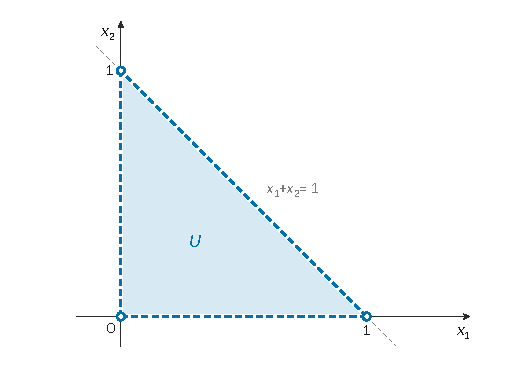
\includegraphics{figures/q5-1-domaine-u.pdf}
\caption*{Figure 1 --- Domaine U pour r = 3 : intérieur du triangle de sommets (0,
0), (1, 0), (0, 1), côtés et sommets exclus}
\end{figure}

\begin{piege}

Le rapport 2026 signale des « Dessins très fantaisistes, tels un quart de cercle, un nuage de points, un trapèze\ldots{} ». Chaque inégalité délimite un demi-plan ; l'intersection des trois est un triangle.

\end{piege}

\hypertarget{question-5.2}{%
\subsection{Question 5.2}\label{question-5.2}}

\begin{indication}{1}

Image réciproque d'un ouvert par une application continue ; intersection finie d'ouverts.

\end{indication}

\begin{indication}{2}

Pour borner, encadrer chaque coordonnée.

\end{indication}

\hypertarget{solution-9}{%
\subsubsection{Solution}\label{solution-9}}

\emph{Ouvert} : \(x\mapsto x_k\) et \(x\mapsto\sum_jx_j\) sont linéaires, donc continues sur \(\mathbb R^{r-1}\).

Les ensembles \(\{x_k>0\}\) et \(\{\sum_jx_j<1\}\) sont des images réciproques d'intervalles ouverts, donc des ouverts. \(U\) est l'intersection de ces \(r\) ouverts.

\emph{Borné} : pour \(x\in U\), \(0<x_k\le\sum_jx_j<1\), donc \(U\subset\,]0,1[^{r-1}\).

\begin{jury}

Le rapport 2026 note que la plupart des candidats prouvent que \(U\) est borné, mais que les justifications de l'ouverture « sont parfois très originales ». L'argument attendu tient en une ligne : image réciproque d'un ouvert par une application continue, puis intersection finie.

\end{jury}

\hypertarget{question-5.3}{%
\subsection{Question 5.3}\label{question-5.3}}

\begin{indication}{1}

Éliminer \(x_r\) grâce à la contrainte ; que devient \(1-x_r\) ?

\end{indication}

\hypertarget{solution-10}{%
\subsubsection{Solution}\label{solution-10}}

La contrainte donne \(x_r=1-\sum_{j<r}x_j\), donc \(1-x_r=\sum_{j<r}x_j\). Pour \((x_1,\dots,x_{r-1})\in U\), on a bien \(x_r\in\,]0,1[\), et
\equationajustee{\begin{aligned}{}&h(x_1,\dots,x_{r-1})\\
&\quad=\sum_{j=1}^{r-1}(1-x_j)^n+\Big(\sum_{j=1}^{r-1}x_j\Big)^n.
\end{aligned}}

\begin{methode}

C'est la façon standard de traiter un extremum sous une contrainte affine. On paramètre l'ensemble des contraintes par \(r-1\) variables libres, sur un \textbf{ouvert}, pour pouvoir utiliser la condition nécessaire \(\nabla h=0\).

\end{methode}

\begin{piege}

Le rapport 2026 constate que « La prise en compte de la contrainte semble totalement leur échapper ». On lit \(h(m)=\sum_{j=1}^r(1-x_j)^r\), avec \(r\) variables et un exposant faux. La fonction \(h\) ne doit dépendre que de \(x_1,\dots,x_{r-1}\) : c'est elle qui conditionne les questions 5.5 et 5.6.

\end{piege}

\hypertarget{question-5.4}{%
\subsection{Question 5.4}\label{question-5.4}}

\begin{indication}{1}

De quel type de fonction s'agit-il ?

\end{indication}

\hypertarget{solution-11}{%
\subsubsection{Solution}\label{solution-11}}

\(h\) est polynomiale en \((x_1,\dots,x_{r-1})\), donc de classe \(\mathcal C^\infty\) sur \(\mathbb R^{r-1}\), a fortiori \(\mathcal C^2\) sur \(U\).

\begin{jury}

Le rapport 2026 regrette des « justifications laborieuses et oiseuses pour ce résultat pourtant très simple : le côté polynomial de h est trop peu souvent évoqué ». Une phrase suffit.

\end{jury}

\hypertarget{question-5.5.1}{%
\subsection{Question 5.5.1}\label{question-5.5.1}}

\begin{indication}{1}

Deux termes dépendent de \(x_j\) : \((1-x_j)^n\) et la puissance de la somme.

\end{indication}

\hypertarget{solution-12}{%
\subsubsection{Solution}\label{solution-12}}

Avec \(s=\sum_kx_k\) :
\equationajustee{\frac{\partial h}{\partial x_j}(m)=-n(1-x_j)^{n-1}+n\,s^{n-1}.}

\begin{piege}

Oublier la contribution de \(s^n\), qui dépend de toutes les variables.

\end{piege}

\begin{jury}

Le rapport 2026 juge cette question et la suivante « en général correctement traitées pour ceux qui ont la bonne fonction h ». Tout se joue donc en 5.3.

\end{jury}

\hypertarget{question-5.5.2}{%
\subsection{Question 5.5.2}\label{question-5.5.2}}

\begin{indication}{1}

Annuler toutes les dérivées partielles ; sur \(U\), les quantités élevées à la puissance \(n-1\) sont strictement positives.

\end{indication}

\begin{indication}{2}

L'injectivité de \(t\mapsto t^{n-1}\) sur \(]0,+\infty[\) montre que tous les \(x_j\) sont égaux.

\end{indication}

\hypertarget{solution-13}{%
\subsubsection{Solution}\label{solution-13}}

Sur \(U\), \(s>0\) et \(1-x_j>0\). La fonction \(t\mapsto t^{n-1}\) est injective sur \(]0,+\infty[\), donc
\equationajustee{\begin{aligned}{}&\nabla h(m)=0\\
\iff\ &\forall j,\ 1-x_j=s.
\end{aligned}}

Tous les \(x_j\) valent donc \(c=1-s\). On en tire \(s=(r-1)c\), puis \(1-c=(r-1)c\), soit \(c=\frac1r\).

Réciproquement, \((\frac1r,\dots,\frac1r)\in U\) annule le gradient. L'unique point critique est \(b=(\frac1r,\dots,\frac1r)\).

\begin{piege}

Pour \(n-1\) pair, \(t\mapsto t^{n-1}\) n'est pas injective sur \(\mathbb R\) : il faut dire que les quantités sont positives.

\end{piege}

\hypertarget{question-5.6.1}{%
\subsection{Question 5.6.1}\label{question-5.6.1}}

\begin{indication}{1}

Dériver le gradient : distinguer \(i=j\) et \(i\ne j\). Puis évaluer en \(b\), où \(s\) et \(1-x_j\) prennent la même valeur.

\end{indication}

\hypertarget{solution-14}{%
\subsubsection{Solution}\label{solution-14}}

\equationajustee{\frac{\partial^2h}{\partial x_i\partial x_j}(m)=n(n-1)s^{n-2}+\delta_{ij}\,n(n-1)(1-x_j)^{n-2}.}
En \(b\), \(s\) et \(1-x_j\) valent tous deux \(\frac{r-1}r\). Posons
\equationajustee{A=n(n-1)\Big(\frac{r-1}r\Big)^{n-2}>0.}
Alors, avec \(J\) la matrice de taille \(r-1\) dont tous les coefficients valent 1 :
\equationajustee{H_h(b)=A\,(I_{r-1}+J).}

\begin{methode}

Reconnaître la matrice des préliminaires (avec \(p=r-1\ge2\), ce qui explique l'hypothèse \(r\ge3\)) : c'est le fil conducteur de l'exercice.

\end{methode}

\begin{piege}

Le rapport 2026 signale qu'« On obtient parfois la matrice nulle ! » ; c'est le symptôme d'une fonction \(h\) fausse. Il relève aussi, dans ses remarques générales, des hessiennes écrites en \(2\times2\) quel que soit le nombre de variables. Ici la matrice est de taille \(r-1\), avec \(r\) quelconque.

\end{piege}

\hypertarget{question-5.6.2}{%
\subsection{Question 5.6.2}\label{question-5.6.2}}

\begin{indication}{1}

Condition suffisante du second ordre : point critique et hessienne définie positive.

\end{indication}

\begin{indication}{2}

Utiliser 3.3 avec la bonne valeur de \(p\), et le signe de \(A\).

\end{indication}

\hypertarget{solution-15}{%
\subsubsection{Solution}\label{solution-15}}

D'après 3.3, \(I_{r-1}+J\in\mathcal S^{++}_{r-1}(\mathbb R)\). Comme \(A>0\), \(H_h(b)\in\mathcal S^{++}_{r-1}(\mathbb R)\).

Les trois hypothèses de la condition suffisante du second ordre sont réunies : \(h\) est \(\mathcal C^2\) sur l'ouvert \(U\), \(b\) est critique, la hessienne y est définie positive. Donc \textbf{\(h\) admet un minimum local strict en \(b\)}.

En ce point, \(x_r=1-\frac{r-1}r=\frac1r\) : \(\mathbb E(X)\) admet un minimum local pour \(x_1=\dots=x_r=\frac1r\).

\begin{jury}

Le rapport 2026 trouve cette question « bien rédigée pour ceux qui l'ont abordée ». La rédaction attendue rappelle explicitement les trois hypothèses (fonction \(\mathcal C^2\), ouvert, point critique) avant de conclure.

\end{jury}

\hypertarget{question-5.6.3}{%
\subsection{Question 5.6.3}\label{question-5.6.3}}

\begin{indication}{1}

Appliquer Jensen avec des poids égaux aux \(r\) nombres \(u_j=1-x_j\) ; calculer leur somme.

\end{indication}

\begin{indication}{2}

Pour le « seulement si », il faut un cas d'égalité. Penser à la position de la courbe d'une fonction strictement convexe par rapport à une de ses tangentes.

\end{indication}

\begin{indication}{3}

Écrire \(\varphi(t)-\varphi(\mu)-\varphi'(\mu)(t-\mu)\) comme une intégrale de \(\varphi'(v)-\varphi'(\mu)\), puis sommer en \(t=u_j\), avec \(\mu\) la moyenne des \(u_j\).

\end{indication}

\hypertarget{solution-16}{%
\subsubsection{Solution}\label{solution-16}}

Soit \((x_j)\in\,]0,1[^r\) avec \(\sum x_j=1\), et \(u_j=1-x_j\in\,]0,1[\). Alors \(\sum_ju_j=r-1\) ; la moyenne des \(u_j\) vaut \(\mu=\frac{r-1}r\).

\emph{Minoration.} Par Jensen à poids \(\frac1r\) :
\equationajustee{\mu^n\le\frac1r\sum_ju_j^n.}
Le membre de droite vaut \(\frac1r\mathbb E(X)\), donc \(\mathbb E(X)\ge r\big(\frac{r-1}r\big)^n\). Cette valeur est atteinte en \(x_j=\frac1r\).

\emph{Égalité.} Posons
\equationajustee{g(t)=\varphi(t)-\varphi(\mu)-\varphi'(\mu)(t-\mu).}
On a \(g(t)=\int_\mu^t(\varphi'(v)-\varphi'(\mu))\,dv\). Comme \(\varphi'\) est strictement croissante, l'intégrande a le signe de \(v-\mu\). Donc \(g(t)>0\) si \(t\ne\mu\), et \(g(\mu)=0\).

Puisque \(\sum_j(u_j-\mu)=0\) :
\equationajustee{\begin{aligned}
\sum_{j=1}^rg(u_j)&=\sum_ju_j^n-r\mu^n-\varphi'(\mu)\sum_j(u_j-\mu)\\
&=\mathbb E(X)-r\Big(\frac{r-1}r\Big)^n.
\end{aligned}}
Une somme de réels positifs est nulle si et seulement si chacun est nul. Donc \(\mathbb E(X)=r\big(\frac{r-1}r\big)^n\) si et seulement si tous les \(u_j\) valent \(\mu\), c'est-à-dire tous les \(x_j\) valent \(\frac1r\).

\textbf{Conclusion} : \(\mathbb E(X)\) est minimale (de minimum \(r\big(\frac{r-1}r\big)^n\)) si et seulement si \(x_1=\dots=x_r=\frac1r\).

\begin{piege}

Écrire « par stricte convexité, il y a égalité si et seulement si les \(u_j\) sont égaux » sans démonstration. Le cas d'égalité de Jensen n'est pas un résultat du cours, et c'est précisément le sens « seulement si » qui est demandé.

\end{piege}

\begin{methode}

Le minimum local de 5.6.2 ne donne rien de global ; la convexité, elle, donne directement un minimum global et son unicité. Les deux approches sont complémentaires.

\end{methode}

\begin{jury}

« Question rarement traitée » selon le rapport 2026. Elle ne demande pourtant que la question 2 et un cas d'égalité : c'est une question qui sépare les bonnes copies.

\end{jury}

\hypertarget{exercice-2-question-de-cours}{%
\section{Exercice 2 --- Question de cours}\label{exercice-2-question-de-cours}}

Deux rappels qui serviront de briques : séries de Riemann (pour toutes les comparaisons) et série géométrique (pour la question 7).

\hypertarget{question-1-1}{%
\subsection{Question 1}\label{question-1-1}}

\begin{indication}{1}

Résultat de cours sur les séries de Riemann.

\end{indication}

\hypertarget{solution-17}{%
\subsubsection{Solution}\label{solution-17}}

\(\sum_{n\ge1}\frac1{n^x}\) converge si et seulement si \(x>1\) ; on note alors \(\zeta(x)\) sa somme.

\begin{piege}

Le rapport 2026 a lu que \(\zeta\) serait définie sur \([2,+\infty[\), voire sur \(]-\infty,1[\cup]1,+\infty[\). Le domaine est \(]1,+\infty[\) : la série diverge pour \(x\le1\).

\end{piege}

\hypertarget{question-2-1}{%
\subsection{Question 2}\label{question-2-1}}

\begin{indication}{1}

Série géométrique : rayon, comportement au bord, somme.

\end{indication}

\hypertarget{solution-18}{%
\subsubsection{Solution}\label{solution-18}}

Le rayon de convergence vaut \(1\), et l'intervalle de convergence est \(]-1,1[\) : divergence grossière en \(1\) et en \(-1\). Pour \(|t|<1\) :
\equationajustee{\sum_{n=0}^{+\infty}t^n=\frac1{1-t}.}

\begin{piege}

Le rapport 2026 relève des intervalles faux (\([0,1[\), \(]-1,1]\)) et des sommes fausses (\(\frac1{1+t}\)) : « on voit toutes les bêtises possibles sur cette question élémentaire ». En \(t=-1\), le terme général \((-1)^n\) ne tend pas vers \(0\).

\end{piege}

\hypertarget{exercice-2-les-fonctions-e_k}{%
\section{\texorpdfstring{Exercice 2 --- Les fonctions \(E_k\)}{Exercice 2 --- Les fonctions E\_k}}\label{exercice-2-les-fonctions-e_k}}

On établit l'existence, la périodicité et la parité. Il faut faire attention au cas \(k=1\), où seules les \textbf{paires} de termes forment une série convergente.

\hypertarget{question-3}{%
\subsection{Question 3}\label{question-3}}

\begin{indication}{1}

Réduire \(\frac1{x-n}+\frac1{x+n}\) au même dénominateur, puis donner un équivalent de sa valeur absolue quand \(n\to+\infty\).

\end{indication}

\hypertarget{solution-19}{%
\subsubsection{Solution}\label{solution-19}}

Pour \(n\ge1\), \(x\pm n\ne0\) car \(x\notin\mathbb Z\), et
\equationajustee{\frac1{x-n}+\frac1{x+n}=\frac{2x}{x^2-n^2}.}
Ce terme change de signe selon \(n\) ; on passe à la valeur absolue :
\equationajustee{\Big|\frac{2x}{x^2-n^2}\Big|\underset{n\to+\infty}{\sim}\frac{2|x|}{n^2}.}
Par comparaison à une série de Riemann convergente, la série converge absolument, donc converge. Comme \(x\ne0\), \textbf{\(E_1(x)\) existe}.

\begin{piege}

Les séries \(\sum\frac1{x-n}\) et \(\sum\frac1{x+n}\) \textbf{divergent} séparément : elles se comportent comme la série harmonique. On ne doit jamais les séparer pour \(k=1\), ni ici ni dans la suite.

\end{piege}

\begin{jury}

Le rapport 2026 : « La convergence absolue n'est presque jamais utilisée ». Il cite une chaîne fausse, \(\frac{2x}{x^2-n^2}\sim\frac{-2x}{n^2}\sim\frac1{n^2}\). Un équivalent ne supprime pas la constante \(-2x\). La comparaison des séries à termes positifs ne s'applique qu'aux valeurs absolues.

\end{jury}

\hypertarget{question-4.1-1}{%
\subsection{Question 4.1}\label{question-4.1-1}}

\begin{indication}{1}

Pour \(k\ge2\), chaque série se traite seule : un équivalent du module du terme général suffit.

\end{indication}

\hypertarget{solution-20}{%
\subsubsection{Solution}\label{solution-20}}

\(\big|\frac1{(x\pm n)^k}\big|\sim\frac1{n^k}\), avec \(k\ge2>1\). Par comparaison de séries à termes positifs, les deux séries convergent absolument.

\begin{piege}

Le rapport 2026 relève l'argument « \(\frac1{(x-n)^k}\sim\frac{(-1)^k}{n^k}\) et le théorème sur les séries alternées permet de conclure ». Ce terme n'alterne pas en \(n\) : \((-1)^k\) ne dépend pas de \(n\). Il faut passer par la convergence absolue.

\end{piege}

\hypertarget{question-4.2-1}{%
\subsection{Question 4.2}\label{question-4.2-1}}

\begin{indication}{1}

Somme d'un terme défini et de deux séries convergentes.

\end{indication}

\hypertarget{solution-21}{%
\subsubsection{Solution}\label{solution-21}}

\(x\ne0\) et les deux séries de 4.1 convergent : \(E_k(x)\) existe pour \(k\ge2\).

Dans toute la suite, on note
\equationajustee{u_{k,n}(x)=\frac1{(x-n)^k}+\frac1{(x+n)^k}.}
Pour \textbf{tout} \(k\ge1\), on a alors \(E_k(x)=\frac1{x^k}+\sum_{n\ge1}u_{k,n}(x)\).

\begin{methode}

Cette écriture unique par paires \(u_{k,n}\) permet de traiter tous les \(k\), y compris \(k=1\), d'un seul coup dans les questions 5 et 6.

\end{methode}

\hypertarget{question-5.1-1}{%
\subsection{Question 5.1}\label{question-5.1-1}}

\begin{indication}{1}

Raisonner sur des sommes partielles \textbf{finies} symétriques, de \(m=-N\) à \(m=N\).

\end{indication}

\begin{indication}{2}

Après le décalage \(x\to x+1\), comparer les deux sommes finies : il reste deux termes « de bord ».

\end{indication}

\hypertarget{solution-22}{%
\subsubsection{Solution}\label{solution-22}}

Pour \(N\ge1\), soit
\equationajustee{\begin{aligned}
S_N(x)&=\frac1{x^k}+\sum_{n=1}^Nu_{k,n}(x)\\
&=\sum_{m=-N}^N\frac1{(x+m)^k}.
\end{aligned}}
On a \(S_N(x)\to E_k(x)\). Par changement d'indice :
\equationajustee{\begin{aligned}
S_N(x+1)&=\sum_{m=-N+1}^{N+1}\frac1{(x+m)^k}\\
&=S_N(x)-\frac1{(x-N)^k}+\frac1{(x+N+1)^k}.
\end{aligned}}
Les termes de bord tendent vers \(0\). À la limite, \(E_k(x+1)=E_k(x)\) pour tout \(x\in\mathbb R\setminus\mathbb Z\) (et \(x+1\in\mathbb R\setminus\mathbb Z\)) : \textbf{\(E_k\) est 1-périodique}.

\begin{piege}

Réindexer directement « la série \(\sum_n\frac1{x+1-n}\) » n'a pas de sens pour \(k=1\) : elle diverge. Sur des sommes finies, toutes les manipulations sont licites ; on ne passe à la limite qu'à la fin.

\end{piege}

\hypertarget{question-5.2-1}{%
\subsection{Question 5.2}\label{question-5.2-1}}

\begin{indication}{1}

Comparer \(u_{k,n}(-x)\) et \(u_{k,n}(x)\), terme apparié par terme apparié.

\end{indication}

\hypertarget{solution-23}{%
\subsubsection{Solution}\label{solution-23}}

\(\mathbb R\setminus\mathbb Z\) est symétrique par rapport à \(0\). Pour \(n\ge1\) :
\equationajustee{\begin{aligned}
u_{k,n}(-x)&=\frac1{(-(x+n))^k}+\frac1{(-(x-n))^k}\\
&=(-1)^ku_{k,n}(x).
\end{aligned}}
De plus, \(\frac1{(-x)^k}=\frac{(-1)^k}{x^k}\). En sommant la série convergente des \(u_{k,n}\) :
\equationajustee{E_k(-x)=(-1)^kE_k(x).}
\textbf{\(E_k\) est paire si \(k\) est pair, impaire si \(k\) est impair.}

\begin{piege}

Pour \(k=1\), écrire \(E_1(-x)\) comme somme de deux séries séparées puis « factoriser », c'est manipuler deux séries divergentes. Le calcul sur les paires évite le problème.

\end{piege}

\begin{jury}

Le rapport 2026 juge ces deux questions (5.1 et 5.2) en général bien traitées. Il cite pourtant une « preuve » de périodicité à proscrire : les \(E_k\) seraient 1-périodiques « puisqu'ils ne contiennent pas des fonctions 2π−périodiques ». Une périodicité se démontre par un calcul.

\end{jury}

\hypertarget{exercice-2-une-relation-de-ruxe9currence}{%
\section{Exercice 2 --- Une relation de récurrence}\label{exercice-2-une-relation-de-ruxe9currence}}

Le théorème de dérivation terme à terme donne \(E_k'=-kE_{k+1}\). Une récurrence en déduit la régularité et l'expression de \(E_k\) par les dérivées de \(E_1\).

\hypertarget{question-6.1}{%
\subsection{Question 6.1}\label{question-6.1}}

\begin{indication}{1}

Théorème de dérivation terme à terme : il porte sur un \textbf{intervalle}. Or \(\mathbb R\setminus\mathbb Z\) n'en est pas un ; découper.

\end{indication}

\begin{indication}{2}

Sur un segment \([\alpha,\beta]\) inclus dans \(]p,p+1[\), minorer \(|x\pm n|\) par \(n/2\) pour \(n\) assez grand, puis majorer \(|u_{k,n}'|\) uniformément.

\end{indication}

\hypertarget{solution-24}{%
\subsubsection{Solution}\label{solution-24}}

Fixons \(k\ge1\), \(p\in\mathbb Z\), et notons \(I_p=\,]p,p+1[\).

\begin{itemize}
\item
  \(u_{k,n}\in\mathcal C^1(I_p)\) et \(u_{k,n}'=-k\,u_{k+1,n}\).
\item
  \(\sum u_{k,n}\) converge simplement sur \(I_p\) (questions 3 et 4).
\item
  Soit \([\alpha,\beta]\subset I_p\) et \(A=\max(|\alpha|,|\beta|)\). Pour \(n\ge2A\), on a \(|x\pm n|\ge n-|x|\ge\frac n2\) sur ce segment.

  Donc \(\sup_{[\alpha,\beta]}|u_{k,n}'|\le\frac{2^{k+2}k}{n^{k+1}}\), terme d'une série convergente car \(k+1\ge2\).

  Ainsi \(\sum u_{k,n}'\) converge normalement, donc uniformément, sur tout segment de \(I_p\).
\end{itemize}

Le théorème de dérivation terme à terme s'applique : \(\sum_nu_{k,n}\) est \(\mathcal C^1\) sur \(I_p\) et se dérive terme à terme. D'où, sur chaque \(I_p\), donc sur \(\mathbb R\setminus\mathbb Z\) :
\equationajustee{\begin{aligned}
E_k'(x)&=-\frac k{x^{k+1}}-k\sum_{n\ge1}u_{k+1,n}(x)\\
&=-k\,E_{k+1}(x).
\end{aligned}}

\begin{methode}

Schéma standard : \textbf{convergence simple} de la série, \textbf{dérivées continues}, \textbf{convergence uniforme (ici normale) de la série des dérivées sur tout segment} de l'intervalle. La convergence n'est pas uniforme au voisinage des entiers ; on ne la demande que sur les segments.

\end{methode}

\begin{jury}

Le rapport 2026 est sévère : « Le théorème de dérivation des séries de fonctions est inconnu pour un candidat sur 2 environ ! ». Il cite une copie pour laquelle la somme serait dérivable « puisque fonction polynôme ». On énonce le théorème, on vérifie chaque hypothèse, et on précise l'intervalle sur lequel on travaille.

\end{jury}

\hypertarget{question-6.2}{%
\subsection{Question 6.2}\label{question-6.2}}

\begin{indication}{1}

Pour la régularité, une récurrence sur l'ordre de dérivation, valable pour \textbf{tous} les \(k\) simultanément.

\end{indication}

\begin{indication}{2}

Pour la formule, une récurrence sur \(k\) utilisant \(E_{k+1}=-\frac1kE_k'\).

\end{indication}

\hypertarget{solution-25}{%
\subsubsection{Solution}\label{solution-25}}

\emph{Régularité.} Notons \(\mathcal P(q)\) : « pour tout \(k\ge1\), \(E_k\in\mathcal C^q(\mathbb R\setminus\mathbb Z)\) ».

\begin{itemize}
\item
  \(\mathcal P(0)\) : chaque \(E_k\) est dérivable (6.1), donc continue.
\item
  Supposons \(\mathcal P(q)\) et fixons \(k\ge1\). D'après 6.1, \(E_k'=-kE_{k+1}\), et \(E_{k+1}\) est \(\mathcal C^q\) par \(\mathcal P(q)\).

  Donc \(E_k'\) est \(\mathcal C^q\), et \(E_k\) est \(\mathcal C^{q+1}\) : \(\mathcal P(q+1)\) est vraie.
\end{itemize}

Ainsi chaque \(E_k\) est \(\mathcal C^\infty\).

\emph{Formule.} Pour \(k=1\), elle se réduit à \(E_1=E_1^{(0)}\). Supposons \(E_k=\frac{(-1)^{k-1}}{(k-1)!}E_1^{(k-1)}\). Alors :
\equationajustee{\begin{aligned}
E_{k+1}&=-\frac1kE_k'\\
&=-\frac1k\cdot\frac{(-1)^{k-1}}{(k-1)!}E_1^{(k)}\\
&=\frac{(-1)^k}{k!}E_1^{(k)}.
\end{aligned}}
Donc \(E_k=\frac{(-1)^{k-1}}{(k-1)!}E_1^{(k-1)}\) pour tout \(k\ge1\).

\begin{piege}

Une récurrence qui ne porterait que sur \(E_1\) (« \(E_1\) est \(\mathcal C^p\) ») oblige à invoquer 6.1 pour \(E_{p+1}\) ; c'est correct, mais il faut le dire. La version « pour tout \(k\) simultanément » ci-dessus est la plus propre.

\end{piege}

\begin{jury}

« La récurrence est souvent mal rédigée » (rapport 2026). On énonce la propriété \(\mathcal P(q)\) avec ses quantificateurs, on vérifie l'initialisation, puis on écrit l'hérédité en citant 6.1.

\end{jury}

\hypertarget{question-7}{%
\subsection{Question 7}\label{question-7}}

\begin{indication}{1}

Faire apparaître une série géométrique de raison \(x/n\).

\end{indication}

\hypertarget{solution-26}{%
\subsubsection{Solution}\label{solution-26}}

On a \(\big|\frac xn\big|\le|x|<1\). Par la question 2, \(\sum_k\frac{x^k}{n^{k+1}}=\frac1n\sum_k\big(\frac xn\big)^k\) converge. Sa somme vaut
\equationajustee{\frac1n\cdot\frac n{n-x}=\frac1{n-x},}
avec \(n-x>0\).

\begin{jury}

Le rapport 2026 : « Le calcul est souvent effectué sans vérifier que \(\left|\frac{x}{n}\right|<1\). » C'est la condition d'application de la question 2 : elle doit figurer dans la copie.

\end{jury}

\hypertarget{question-8}{%
\subsection{Question 8}\label{question-8}}

\begin{indication}{1}

Appliquer 7 en \(x\) et en \(-x\), puis soustraire.

\end{indication}

\begin{indication}{2}

Que deviennent les termes d'indice pair ? Réindexer les impairs par \(k=2s-1\).

\end{indication}

\hypertarget{solution-27}{%
\subsubsection{Solution}\label{solution-27}}

Pour \(n\ge1\) :
\equationajustee{\begin{aligned}
\frac1{n-x}-\frac1{n+x}&=\sum_{k\ge0}\frac{(1-(-1)^k)x^k}{n^{k+1}}\\
&=\sum_{s\ge1}\frac{2x^{2s-1}}{n^{2s}},
\end{aligned}}
les termes d'indice pair étant nuls.

Le membre de gauche, égal à \(\frac{2x}{n^2-x^2}=O(1/n^2)\), est le terme général d'une série convergente. En sommant sur \(n\) :
\equationajustee{\begin{aligned}{}&\sum_{n\ge1}\Big(\frac1{n-x}-\frac1{n+x}\Big)\\
&\qquad=\sum_{n\ge1}\sum_{s\ge1}\frac2{n^{2s}}x^{2s-1}.
\end{aligned}}

\begin{methode}

Aucune interversion n'est faite ici : on somme sur \(n\) une égalité établie pour chaque \(n\). L'interversion est le travail de la question suivante.

\end{methode}

\begin{jury}

Le rapport 2026 place ici sa remarque sur Fubini : le théorème est « vaguement invoqué sous la forme « Fubini positif » ou « Fubini module » » sans hypothèses. Dans la rédaction ci-dessus, la question 8 n'en a pas besoin. En revanche, dès qu'on intervertit (question 9), il faut l'énoncer et en vérifier les hypothèses.

\end{jury}

\hypertarget{question-9}{%
\subsection{Question 9}\label{question-9}}

\begin{indication}{1}

Relier le membre de gauche de 8 à \(E_1(x)\), puis échanger l'ordre des deux sommations pour faire apparaître \(\zeta(2s)\).

\end{indication}

\begin{indication}{2}

Le théorème adapté est celui de Fubini pour les séries doubles ; son hypothèse porte sur les \textbf{valeurs absolues}.

\end{indication}

\begin{indication}{3}

Pour \(n\) fixé, \(\sum_s|a_{n,s}|\) est une série géométrique : calculer sa somme et la majorer par une constante fois \(\frac1{n^2}\).

\end{indication}

\hypertarget{solution-28}{%
\subsubsection{Solution}\label{solution-28}}

On a \(\frac1{x-n}+\frac1{x+n}=-\big(\frac1{n-x}-\frac1{n+x}\big)\). La question 8 donne donc
\equationajustee{\begin{aligned}
E_1(x)&=\frac1x-\sum_n\sum_sa_{n,s},\\
a_{n,s}&=\frac{2x^{2s-1}}{n^{2s}}.
\end{aligned}}

\textbf{Théorème de Fubini pour les séries doubles.} Soit \((a_{n,s})_{(n,s)\in\mathbb N^*\times\mathbb N^*}\) une famille de complexes. On suppose que, pour tout \(n\), \(\sum_s|a_{n,s}|\) converge, et que \(\sum_n\sum_{s=1}^{+\infty}|a_{n,s}|\) converge.

Alors la famille est sommable, et toutes les séries \(\sum_na_{n,s}\) et \(\sum_sa_{n,s}\) convergent. De plus, \(\sum_n\sum_sa_{n,s}=\sum_s\sum_na_{n,s}\).

\textbf{Hypothèses.} Pour \(n\ge1\), \(\sum_s|a_{n,s}|\) est une série géométrique de raison \(\frac{x^2}{n^2}<1\) :
\equationajustee{\begin{aligned}
\sum_{s\ge1}|a_{n,s}|&=\frac{2|x|}{n^2}\cdot\frac1{1-x^2/n^2}\\
&=\frac{2|x|}{n^2-x^2}\\
&\le\frac{2|x|}{(1-x^2)\,n^2}.
\end{aligned}}
Comme \(\sum_n\frac1{n^2}\) converge, les hypothèses sont satisfaites.

\textbf{Conclusion.} \(\sum_na_{n,s}=2x^{2s-1}\zeta(2s)\). D'où, pour \(x\in\,]-1,1[\setminus\{0\}\) :
\equationajustee{E_1(x)=\frac1x-2\sum_{s=1}^{+\infty}\zeta(2s)\,x^{2s-1}.}

\begin{piege}

Intervertir les deux sommes sans vérifier la sommabilité : le résultat est juste, mais la question porte précisément sur la justification. L'énoncé demande de citer le théorème « avec précision ».

\end{piege}

\begin{methode}

Autre majoration possible : \(\sum_n|a_{n,s}|=2|x|^{2s-1}\zeta(2s)\le2\zeta(2)|x|^{2s-1}\), puis sommer en \(s\). Pour des termes positifs, on peut vérifier la sommabilité dans l'ordre de sommation que l'on préfère.

\end{methode}

\begin{jury}

« Peu de réussite sur ces deux dernières questions » (8 et 9), note le rapport 2026. Dans ses remarques générales, il observe que l'énoncé des théorèmes d'inversion est « assez peu maîtrisé, encore moins la vérification des hypothèses ».

\end{jury}

\hypertarget{question-10}{%
\subsection{Question 10}\label{question-10}}

\begin{indication}{1}

Combiner 6.2 et 9 : dériver \(k-1\) fois l'égalité de 9.

\end{indication}

\begin{indication}{2}

Il faut savoir que la série entière \(\sum\zeta(2s)x^{2s-1}\) peut être dérivée terme à terme sur \(]-1,1[\) : que dit la question 9 de son rayon de convergence ?

\end{indication}

\begin{indication}{3}

Exprimer la dérivée \((k-1)\)-ième de \(x^{2s-1}\) à l'aide d'un coefficient binomial, en traitant à part les monômes de degré \(<k-1\).

\end{indication}

\hypertarget{solution-29}{%
\subsubsection{Solution}\label{solution-29}}

Soit \(g(x)=\sum_{s\ge1}\zeta(2s)x^{2s-1}\). La série converge en tout point de \(]-1,1[\) (question 9) : son rayon vérifie \(R\ge1\). Donc \(g\) est \(\mathcal C^\infty\) sur \(]-1,1[\) et se dérive terme à terme :
\equationajustee{g^{(q)}(x)=q!\sum_{s\ge1}\binom{2s-1}{q}\zeta(2s)\,x^{2s-1-q}.}
En effet, si \(q\le2s-1\) :
\equationajustee{\begin{aligned}
(x^{2s-1})^{(q)}&=\frac{(2s-1)!}{(2s-1-q)!}x^{2s-1-q}\\
&=q!\binom{2s-1}qx^{2s-1-q}.
\end{aligned}}
Sinon, cette dérivée est nulle, ce que traduit la convention \(\binom{2s-1}q=0\).

Sur \(]-1,0[\) et sur \(]0,1[\), \(E_1=\frac1x-2g\). On dérive \(k-1\) fois, avec \(\big(\frac1x\big)^{(k-1)}=\frac{(-1)^{k-1}(k-1)!}{x^k}\) :
\equationajustee{E_1^{(k-1)}(x)=\frac{(-1)^{k-1}(k-1)!}{x^k}-2(k-1)!\sum_{s\ge1}\binom{2s-1}{k-1}\zeta(2s)x^{2s-k}.}
Par 6.2, on multiplie par \(\frac{(-1)^{k-1}}{(k-1)!}\). Avec \(-(-1)^{k-1}=(-1)^k\), pour \(x\in\,]-1,1[\), \(x\ne0\) :
\equationajustee{E_k(x)=\frac1{x^k}+2(-1)^k\sum_{s=1}^{+\infty}\binom{2s-1}{k-1}\zeta(2s)\,x^{2s-k}.}

\begin{piege}

Invoquer la « règle de Cauchy » (\(\zeta(2s)^{1/(2s-1)}\to1\)) pour le rayon de convergence : elle n'est pas au programme, et elle est inutile puisque la question 9 donne déjà la convergence sur \(]-1,1[\).

\end{piege}

\begin{methode}

Contrôle rapide : pour \(k=1\), on retrouve la question 9 ; pour \(k=2\), la formule redonne \(E_2=-E_1'\) en dérivant terme à terme. Vérifier ainsi un ou deux cas particuliers évite les erreurs de signe.

\end{methode}

\hypertarget{exercice-3-cas-mathbb-kmathbb-r}{%
\section{\texorpdfstring{Exercice 3 --- Cas \(\mathbb K=\mathbb R\)}{Exercice 3 --- Cas \textbackslash mathbb K=\textbackslash mathbb R}}\label{exercice-3-cas-mathbb-kmathbb-r}}

On explicite la diagonalisation d'une matrice symétrique réelle de rang 2 : noyau de dimension \(n-2\), puis deux valeurs propres non nulles, racines d'un trinôme.

Notations : \(\sigma=\sum_{j=1}^{n-1}a_j^2\) ; \((e_1,\dots,e_n)\) est la base canonique ; \(F_\lambda=\ker(M-\lambda I_n)\).

\hypertarget{question-1.1}{%
\subsection{Question 1.1}\label{question-1.1}}

\begin{indication}{1}

Regarder la transposée de \(M\).

\end{indication}

\hypertarget{solution-30}{%
\subsubsection{Solution}\label{solution-30}}

Pour \(i<n\), \(M_{i,n}=a_i=M_{n,i}\), et les autres coefficients hors de la dernière ligne et de la dernière colonne sont nuls : \(M^T=M\).

Les \(a_j\) sont réels : \(M\) est symétrique \textbf{réelle}, donc diagonalisable (en base orthonormée) par le théorème spectral.

\begin{jury}

Le rapport 2026 : « Comme d'habitude un grand nombre de copies oublient de souligner le caractère « réel » des coefficients. » Sans ce mot, l'argument est faux : la partie 2 exhibe une matrice symétrique complexe non diagonalisable.

\end{jury}

\hypertarget{question-1.2}{%
\subsection{Question 1.2}\label{question-1.2}}

\begin{indication}{1}

Décrire les colonnes : les \(n-1\) premières sont toutes colinéaires à un même vecteur.

\end{indication}

\begin{indication}{2}

Utiliser \(a_1\ne0\) pour exhiber deux colonnes non colinéaires.

\end{indication}

\hypertarget{solution-31}{%
\subsubsection{Solution}\label{solution-31}}

Pour \(j<n\), \(C_j=a_je_n\), et \(C_n=(a_1,\dots,a_n)^T\). Donc \(\mathrm{Im}\,M\subset\mathrm{Vect}(e_n,C_n)\), et \(\mathrm{rg}\,M\le2\).

Comme \(C_1=a_1e_n\ne0\), et que \(C_n\), de première coordonnée \(a_1\ne0\), n'est pas colinéaire à \(e_n\), la famille \((C_1,C_n)\) est libre. Donc \(\mathrm{rg}\,M=2\).

\begin{piege}

Le rang ne dépend que de \(a_1\ne0\) : si \(a_1=\dots=a_{n-1}=0\), le rang tomberait à \(1\) ou \(0\). C'est la seule hypothèse qui intervient.

\end{piege}

\begin{jury}

Le rapport 2026 : « rg(M) = 2 n'est pas prouvé par un candidat sur deux. » Il faut les deux inégalités : la majoration par les colonnes, puis une famille libre de deux colonnes.

\end{jury}

\hypertarget{question-1.3}{%
\subsection{Question 1.3}\label{question-1.3}}

\begin{indication}{1}

Théorème du rang, puis lien entre multiplicité et dimension du sous-espace propre pour une matrice diagonalisable.

\end{indication}

\hypertarget{solution-32}{%
\subsubsection{Solution}\label{solution-32}}

Par le théorème du rang, \(\dim\ker M=n-2\ge1\) : \(0\) est valeur propre.

\(M\) étant diagonalisable, la multiplicité de \(0\) comme racine de \(\chi_M\) est égale à \(\dim\ker M\) : \textbf{multiplicité \(n-2\)}.

\begin{piege}

L'égalité « multiplicité \(=\) dimension du sous-espace propre » n'est vraie en général que dans un sens (dimension \(\le\) multiplicité). Ici, c'est la diagonalisabilité (1.1) qui donne l'égalité : il faut la citer.

\end{piege}

\begin{jury}

Selon le rapport 2026, « la plupart ne connaissent pas la différence entre ordre de multiplicité de la valeur propre 0 et dimension de son sous-espace vectoriel propre associé ». Il cite aussi des confusions entre \(\dim\mathcal M_n(\mathbb R)=n^2\) et \(n\) dans le théorème du rang. Le théorème du rang porte sur l'endomorphisme de \(\mathbb R^n\) associé à \(M\).

\end{jury}

\hypertarget{question-1.4}{%
\subsection{Question 1.4}\label{question-1.4}}

\begin{indication}{1}

Pour une matrice diagonalisable, les multiplicités des valeurs propres totalisent \(n\).

\end{indication}

\hypertarget{solution-33}{%
\subsubsection{Solution}\label{solution-33}}

\(\chi_M\) est scindé (car \(M\) est diagonalisable), de degré \(n\). Le réel \(0\) y est racine de multiplicité exactement \(n-2\). Les deux racines restantes, comptées avec multiplicité, sont donc non nulles :
\equationajustee{\chi_M=X^{n-2}(X-\lambda_1)(X-\lambda_2),}
avec \(\lambda_1\neq0\) et \(\lambda_2\neq0\).

\begin{jury}

« Réponse souvent très mal justifiée : beaucoup de verbiage » (rapport 2026). Trois arguments suffisent : \(\chi_M\) scindé, degré \(n\), multiplicité exacte de \(0\).

\end{jury}

\hypertarget{question-1.5}{%
\subsection{Question 1.5}\label{question-1.5}}

\begin{indication}{1}

Résoudre \(MX=0\) ligne par ligne : que disent les \(n-1\) premières lignes ?

\end{indication}

\begin{indication}{2}

Il reste une seule équation linéaire en \(x_1,\dots,x_{n-1}\) ; chercher des vecteurs simples qui la vérifient, sans dénominateur.

\end{indication}

\hypertarget{solution-34}{%
\subsubsection{Solution}\label{solution-34}}

Les lignes \(i<n\) donnent \(a_ix_n=0\), donc \(x_n=0\) (car \(a_1\ne0\)). La dernière ligne donne alors \(\sum_{j<n}a_jx_j=0\). Ainsi :
\equationajustee{\begin{aligned}
\ker M=\big\{X:\ &x_n=0\\
\text{et }\ &\textstyle\sum_{j<n}a_jx_j=0\big\}.
\end{aligned}}

Pour \(2\le k\le n-1\), le vecteur \(v_k=a_ke_1-a_1e_k\) est dans \(\ker M\).

Les \(n-2\) vecteurs \(v_2,\dots,v_{n-1}\) sont libres : seul \(v_k\) a une coordonnée d'indice \(k\) non nulle, égale à \(-a_1\). Comme \(\dim\ker M=n-2\) :
\equationajustee{\ker M=\mathrm{Vect}(v_2,\dots,v_{n-1}).}

\begin{methode}

Pour un hyperplan d'équation \(\sum_ja_jx_j=0\) avec \(a_1\ne0\), les vecteurs \(a_ke_1-a_1e_k\) en donnent toujours une base, sans fraction.

\end{methode}

\begin{jury}

Le rapport 2026 : « Beaucoup de candidats n'arrivent pas à mener à termes ces calculs plutôt simples. » Il revient, dans ses remarques générales, sur la recherche d'une base du noyau d'une matrice de rang 2. Une fois la dimension connue (1.3), il suffit d'exhiber \(n-2\) vecteurs libres du noyau.

\end{jury}

\hypertarget{question-1.6}{%
\subsection{Question 1.6}\label{question-1.6}}

\begin{indication}{1}

Les \(n-1\) premières lignes de \(MX=\lambda X\) expriment chaque \(x_i\) en fonction de \(x_n\), puisque \(\lambda\ne0\).

\end{indication}

\begin{indication}{2}

Montrer que \(x_n\ne0\), puis reporter dans la dernière ligne.

\end{indication}

\hypertarget{solution-35}{%
\subsubsection{Solution}\label{solution-35}}

Pour \(i<n\), la ligne \(i\) donne \(a_ix_n=\lambda x_i\), d'où \(x_i=\frac{a_i}\lambda x_n\).

Si \(x_n=0\), tous les \(x_i\) sont nuls et \(X=0\) : exclu. Donc \(x_n\ne0\).

La dernière ligne s'écrit \(\frac\sigma\lambda x_n+a_nx_n=\lambda x_n\). En divisant par \(x_n\) et en multipliant par \(\lambda\) :
\equationajustee{\lambda^2-\lambda a_n-\sigma=0.}
\(\lambda_1\) et \(\lambda_2\) sont des valeurs propres non nulles : elles vérifient cette équation.

Le discriminant vaut \(\Delta=a_n^2+4\sigma\ge4a_1^2>0\), et le produit des racines \(-\sigma<0\). Les racines sont réelles, distinctes, de signes opposés :
\equationajustee{\lambda_1=\frac{a_n-\sqrt{a_n^2+4\sigma}}2<0<\lambda_2=\frac{a_n+\sqrt{a_n^2+4\sigma}}2.}
Comme \(\lambda_1,\lambda_2\) (comptées avec multiplicité) sont racines de ce trinôme à racines simples, ce sont exactement ces deux racines.

\begin{piege}

L'énoncé dit « éventuellement égales » en 1.4 ; sur \(\mathbb R\), elles ne le sont jamais. Ce sera la différence essentielle avec le cas complexe.

\end{piege}

\hypertarget{question-1.7}{%
\subsection{Question 1.7}\label{question-1.7}}

\begin{indication}{1}

L'analyse de 1.6 donne la forme de tout vecteur propre ; choisir \(x_n\) pour éliminer les dénominateurs, puis vérifier.

\end{indication}

\hypertarget{solution-36}{%
\subsubsection{Solution}\label{solution-36}}

Soit \(\lambda\in\{\lambda_1,\lambda_2\}\). Par 1.6, tout vecteur de \(F_\lambda\) est proportionnel à \(w_\lambda=(a_1,\dots,a_{n-1},\lambda)^T\) (prendre \(x_n=\lambda\)).

Réciproquement, \((Mw_\lambda)_i=a_i\lambda\) pour \(i<n\). Pour la dernière coordonnée :
\equationajustee{\begin{aligned}
(Mw_\lambda)_n&=\sigma+a_n\lambda\\
&=\lambda^2.
\end{aligned}}
Donc \(Mw_\lambda=\lambda w_\lambda\), et
\equationajustee{\begin{aligned}
F_{\lambda_1}&=\mathrm{Vect}\big((a_1,\dots,a_{n-1},\lambda_1)^T\big),\\
F_{\lambda_2}&=\mathrm{Vect}\big((a_1,\dots,a_{n-1},\lambda_2)^T\big).
\end{aligned}}

\begin{jury}

Le rapport 2026 constate « de la réussite pour les rares candidats » qui ont traité 1.7 et 1.8. Ces deux questions sont accessibles dès que 1.5 et 1.6 sont faites.

\end{jury}

\hypertarget{question-1.8}{%
\subsection{Question 1.8}\label{question-1.8}}

\begin{indication}{1}

Concaténer les bases des trois sous-espaces propres ; justifier que l'on obtient une base de \(\mathbb R^n\).

\end{indication}

\hypertarget{solution-37}{%
\subsubsection{Solution}\label{solution-37}}

Les sous-espaces propres associés à \(0,\lambda_1,\lambda_2\), deux à deux distinctes, sont en somme directe. Leurs dimensions \(n-2,1,1\) ont pour somme \(n\). Soit \(P\) la matrice de colonnes \(v_2,\dots,v_{n-1},w_{\lambda_1},w_{\lambda_2}\) :
\equationajustee{P=\begin{pmatrix}
a_2&a_3&\cdots&a_{n-1}&a_1&a_1\\
-a_1&0&\cdots&0&a_2&a_2\\
0&-a_1&\cdots&0&a_3&a_3\\
\vdots&&\ddots&\vdots&\vdots&\vdots\\
0&0&\cdots&-a_1&a_{n-1}&a_{n-1}\\
0&0&\cdots&0&\lambda_1&\lambda_2
\end{pmatrix}.}
\(P\) est inversible, et
\equationajustee{P^{-1}MP=\mathrm{diag}\Big(\underbrace{0,\dots,0}_{n-2},\ \frac{a_n-\sqrt{a_n^2+4\sigma}}2,\ \frac{a_n+\sqrt{a_n^2+4\sigma}}2\Big).}

\begin{jury}

L'énoncé précise : « On précisera la matrice diagonale obtenue ». Il faut donner les valeurs explicites de \(\lambda_1\) et \(\lambda_2\) et respecter l'ordre des colonnes de \(P\).

\end{jury}

\hypertarget{exercice-3-cas-mathbb-kmathbb-c}{%
\section{\texorpdfstring{Exercice 3 --- Cas \(\mathbb K=\mathbb C\)}{Exercice 3 --- Cas \textbackslash mathbb K=\textbackslash mathbb C}}\label{exercice-3-cas-mathbb-kmathbb-c}}

Une matrice symétrique complexe n'est pas forcément diagonalisable. Il faut calculer \(\chi_M\) et comparer, valeur propre par valeur propre, multiplicité et dimension du sous-espace propre.

\hypertarget{question-2.1}{%
\subsection{Question 2.1}\label{question-2.1}}

\begin{indication}{1}

Commencer par le polynôme caractéristique. Pour \(X\ne0\), une opération sur les colonnes de \(XI_n-M\) la rend triangulaire.

\end{indication}

\begin{indication}{2}

Les résultats de 1.2, 1.5 et 1.6 restent vrais sur \(\mathbb C\) : ils ne reposent que sur \(a_1\ne0\). Ils donnent la dimension de chaque sous-espace propre.

\end{indication}

\begin{indication}{3}

Discuter selon que \(\sigma\) est nul ou non, puis selon le discriminant du trinôme.

\end{indication}

\hypertarget{solution-38}{%
\subsubsection{Solution}\label{solution-38}}

\emph{Polynôme caractéristique.} Soit \(X\ne0\). Dans \(XI_n-M\), la colonne \(j<n\) vaut \(Xe_j-a_je_n\). On effectue \(C_n\leftarrow C_n+\sum_{j<n}\frac{a_j}XC_j\).

La dernière colonne devient \(\big(X-a_n-\frac\sigma X\big)e_n\), et la matrice devient triangulaire inférieure. Avec \(Q=X^2-a_nX-\sigma\) :
\equationajustee{\begin{aligned}
\chi_M(X)&=X^{n-1}\Big(X-a_n-\frac\sigma X\Big)\\
&=X^{n-2}Q(X).
\end{aligned}}
Deux polynômes égaux en une infinité de points sont égaux : l'égalité vaut pour tout \(X\).

\emph{Dimensions.} Sur \(\mathbb C\), \(\dim\ker M=n-2\), et \(\dim F_\lambda=1\) pour toute valeur propre \(\lambda\ne0\). Comme \(\chi_M\) est scindé, \(M\) est diagonalisable si et seulement si chaque sous-espace propre a pour dimension la multiplicité de la valeur propre.

\begin{itemize}
\item
  \(\sigma=0\) : \(Q=X(X-a_n)\). La multiplicité de \(0\) est au moins \(n-1\), alors que \(\dim\ker M=n-2\) : \textbf{non diagonalisable}.
\item
  \(\sigma\ne0\) et \(a_n^2+4\sigma=0\) : racine double \(\mu=\frac{a_n}2\), non nulle car \(Q(0)=-\sigma\ne0\).

  Elle est de multiplicité 2, mais \(\dim F_\mu=1\) : \textbf{non diagonalisable}.
\item
  \(\sigma\ne0\) et \(a_n^2+4\sigma\ne0\) : deux racines simples non nulles distinctes, et \(0\) de multiplicité exactement \(n-2\).

  Les dimensions totalisent \((n-2)+1+1=n\) : \textbf{diagonalisable}.
\end{itemize}

D'où : \(M\) n'est pas diagonalisable si et seulement si \(\sum_{j<n}a_j^2=0\) ou \(a_n^2+4\sum_{j<n}a_j^2=0\).

\begin{piege}

Sur \(\mathbb C\), \(\sum a_j^2=0\) n'entraîne pas \(a_j=0\) (par exemple \(1^2+i^2=0\)). C'est exactement ce qui fait échouer la diagonalisation : ne pas transposer les réflexes du cas réel.

\end{piege}

\begin{methode}

Pour une matrice « en flèche », l'opération sur les colonnes \(C_n\leftarrow C_n+\sum_j\frac{a_j}XC_j\) donne le polynôme caractéristique en une ligne. On évite ainsi le complément de Schur, qui n'est pas au programme.

\end{methode}

\begin{jury}

« Question abordée par très peu de copies » (rapport 2026). C'est la question la plus longue de l'exercice, mais elle réutilise presque tout le cas réel : une copie qui a traité 1.2, 1.5 et 1.6 a déjà les dimensions des sous-espaces propres.

\end{jury}

\hypertarget{question-2.2}{%
\subsection{Question 2.2}\label{question-2.2}}

\begin{indication}{1}

Choisir \(a_1,a_2\) complexes avec \(a_1\ne0\) et \(a_1^2+a_2^2=0\) ; le plus simple est de prendre aussi \(a_3=0\).

\end{indication}

\hypertarget{solution-39}{%
\subsubsection{Solution}\label{solution-39}}

On prend \(a_1=1\), \(a_2=i\), \(a_3=0\) :
\equationajustee{M=\begin{pmatrix}0&0&1\\0&0&i\\1&i&0\end{pmatrix}.}
Ici \(\sigma=0\), donc par 2.1, \(M\) n'est pas diagonalisable.

Directement : \(\chi_M=X^3\), et \(0\) est la seule valeur propre. Diagonalisable, \(M\) serait semblable à la matrice nulle, donc nulle, ce qui est faux. On vérifie d'ailleurs que \(M^3=0\) et que \(M^2\neq0\) :
\equationajustee{M^2=\begin{pmatrix}1&i&0\\i&-1&0\\0&0&0\end{pmatrix}.}

Exemple relevant de la seconde condition : \(a=(1,0,2i)\). Alors \(\sigma=1\) et \(a_3^2+4\sigma=0\) ; on trouve \(\chi_M=X(X-i)^2\) et \(\dim F_i=1\).

\begin{jury}

« Beaucoup d'étudiants donnent un exemple juste » (rapport 2026), même sans avoir traité 2.1. Un exemple se justifie toutefois : on vérifie l'hypothèse \(a_1\ne0\) et l'une des deux conditions.

\end{jury}

\hypertarget{bilan}{%
\section{Bilan}\label{bilan}}

\textbf{Méthodes à retenir}

\begin{itemize}
\tightlist
\item
  Convexité par le signe de \(\varphi''\) ; inégalité de Jensen, et son \textbf{cas d'égalité} démontré par l'inégalité de la tangente (écart à la tangente écrit comme une intégrale de \(\varphi'(v)-\varphi'(\mu)\)).
\item
  Polynôme annulateur \(\Rightarrow\) inclusion du spectre ; matrice symétrique réelle définie positive \(\iff\) spectre dans \(]0,+\infty[\).
\item
  Comptage par indicatrices et linéarité de l'espérance, sans indépendance.
\item
  Extremum sous contrainte affine : élimination d'une variable, ouvert, gradient, hessienne, condition suffisante du second ordre. Puis argument global (convexité) pour passer du local au global.
\item
  Séries de fonctions : regroupement par paires quand les séries séparées divergent ; sommes partielles finies pour les réindexations ; dérivation terme à terme sur chaque \textbf{intervalle}, avec convergence normale des dérivées sur les segments.
\item
  Interversion de sommes : théorème de Fubini pour les séries doubles, sommabilité vérifiée sur les valeurs absolues.
\item
  Réduction : rang par les colonnes, théorème du rang, multiplicités et dimensions des sous-espaces propres ; calcul de \(\chi_M\) par opérations élémentaires.
\end{itemize}

\textbf{Ce que retient le rapport 2026} : une moyenne de 5,68 sur 20, et un rappel général, « une affirmation sans démonstration n'a aucune valeur ». Les questions qui ont fait la différence sont celles listées dans la présentation : Jensen, \(J\) et \(I_p+J\), la fonction \(h\), le minimum global, la dérivation terme à terme, Fubini, le rang de \(M\) et la multiplicité de \(0\), le cas complexe. Le jury insiste aussi sur la présentation (numérotation respectée, copie lisible), qui compte dans le barème.

\textbf{Prérequis à revoir} : théorème spectral et caractérisation de \(\mathcal S_n^{++}\) ; conditions d'ordre 1 et 2 pour les extrema ; théorèmes de régularité des séries de fonctions et des séries entières ; familles sommables ; critère de diagonalisabilité par les dimensions des sous-espaces propres.

\textbf{Questions classiques transposables} : problème du « collectionneur » (nombre d'issues manquantes après \(n\) tirages) ; développement de \(\pi\cot(\pi x)\) et valeurs \(\zeta(2s)\) ; matrices de rang 2 et matrices « en flèche » ; matrices symétriques complexes non diagonalisables (une matrice symétrique complexe nilpotente non nulle en est l'exemple type).

\end{document}
